\section{Auswertung}
\label{sec:Auswertung}

Die Graphen wurden sowohl mit Matplotlib \cite{matplotlib} als auch NumPy \cite{numpy} erstellt.

\subsection{Bestimmung von RC mithilfe des Entladevorgangs des Kondensators}
\label{subsec:1}
\begin{figure}
	\centering
	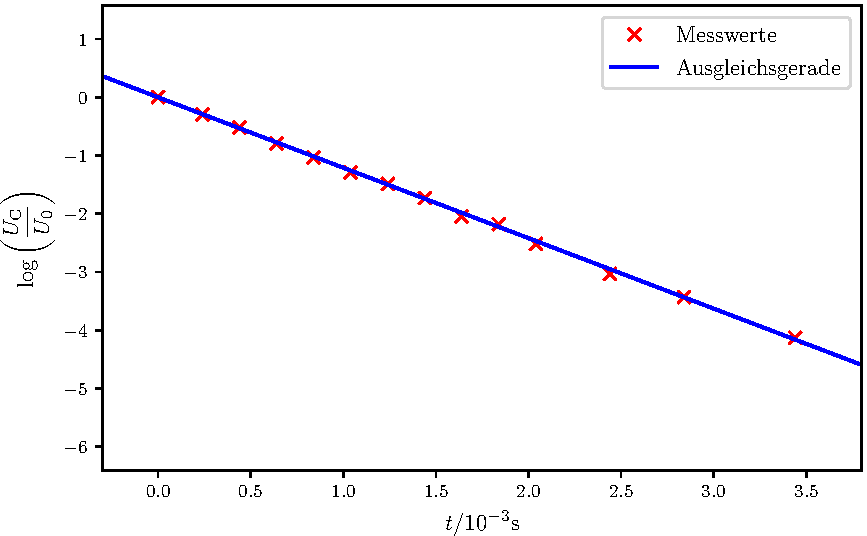
\includegraphics[width=\linewidth-70pt,height=\textheight-70pt,keepaspectratio]{content/images/Graph1.pdf}
	\caption{Die normierte logarithmische Kondensatorspannung $\mathrm{log}\left(\frac{U_.C}{U_.0}\right)$ in Abhängigkeit von der Zeit $t$.}
	\label{fig:Graph1}
\end{figure}

\noindent Nach Formel \eqref{eq:Q1} ergibt sich mit Formel \eqref{eq:QC}:
\[
\mathrm{log}\left(\frac{U_.C}{U_.0}\right) = -\frac{1}{\tau}t 
\]
Dabei beträgt die Spannung $U_.0 = \SI{49.6}{\volt}$.
Eine lineare Ausgleichsrechnung dieser Form liefert mit den Werten aus Tabelle \ref{tab:a} für die Zeitkonstante $\tau$:
\[
\tau = RC = \SI{8.27(7)e-4}{\second}\text{.}
\]
Der Graph ist in Abbildung \ref{fig:Graph1} dargestellt.

\begin{table}
	\centering
	\caption{Die Messwerte für die Zeit $t$, die Spannung $U_.C$, sowie die berechneten Werte für $\mathrm{log}\left(\frac{U_.C}{U_.0}\right)$.}
	\label{tab:taba}
	\sisetup{table-format=1.2}
	\begin{tabular}{S[table-format=1.1]S[table-format=1.2]S[table-format=1.2]}
		\toprule
		{$r/\si{\centi\metre}$} & {$I/\si[per-mode=reciprocal]{\ampere}$} & {$B/\si[per-mode=reciprocal]{\milli\tesla}$} \\
		\midrule
		4.6 & 1.25 & 1.70 \\
		5.1 & 1.39 & 1.88 \\
		5.6 & 1.49 & 2.02 \\
		6.1 & 1.61 & 2.18 \\
		6.6 & 1.71 & 2.32 \\
		7.1 & 1.81 & 2.45 \\
		7.6 & 1.95 & 2.64 \\
		8.1 & 2.09 & 2.83 \\
		8.6 & 2.19 & 2.97 \\
		9.1 & 2.29 & 3.11 \\
		\bottomrule
	\end{tabular}

	\label{tab:a}
\end{table}

\subsection{Bestimmung von RC mithilfe der Amplitude}
\label{subsec:2}
Eine nichtlineare Ausgleichsrechnung nach Formel \eqref{eq:A2} ergibt mit $U_.0 = \SI{96.0}{\volt}$ und den Werten aus Tabelle \ref{tab:b}:
\[
\tau = RC = \SI{5.25(8)e-3}{\second}\text{.}
\]
%Der Graph ist in Abbildung \ref{fig:Graph2} dargestellt.

\begin{table}
	\centering
	\caption{Die Messwerte für die Frequenz $f$, die Amplitude $A$ und die Verschiebung $a$, sowie die berechneten Werte für $\frac{A}{U_.0}$ und die Phasenverschiebung $\phi$.}
	\label{tab:tabb}
	\sisetup{table-format=1.2}
	\begin{tabular}{S[table-format=5.0]S[table-format=2.2]S[table-format=2.2]S[table-format=1.2]S[table-format=1.2]}
		\toprule
		{$f/\si{\hertz}$} & {$U/\si{\volt}$} & {$\frac{U}{U_0}$} & {$a/10^{-4}\si{\second}$} & {$\phi/\si{\radian}$} \\
		\midrule
		   10 & 96.00 & 1.00 & 6.00 & 0.04 \\
		   30 & 94.00 & 0.98 & 6.00 & 0.11 \\
		   70 & 90.00 & 0.94 & 6.00 & 0.26 \\
		  100 & 86.00 & 0.90 & 7.60 & 0.48 \\
		  200 & 66.40 & 0.69 & 6.20 & 0.78 \\
		  300 & 52.00 & 0.54 & 5.20 & 0.98 \\
		  500 & 34.40 & 0.36 & 3.00 & 0.94 \\
		  700 & 25.20 & 0.26 & 3.00 & 1.32 \\
		 1000 & 17.40 & 0.18 & 2.30 & 1.45 \\
		 2000 & 8.00 & 0.08 & 1.20 & 1.51 \\
		 3000 & 4.88 & 0.05 & 0.78 & 1.47 \\
		 4000 & 3.28 & 0.03 & 0.59 & 1.48 \\
		 5000 & 2.24 & 0.02 & 0.47 & 1.48 \\
		 6000 & 1.64 & 0.02 & 0.40 & 1.51 \\
		 7000 & 1.20 & 0.01 & 0.34 & 1.50 \\
		 8000 & 0.84 & 0.01 & 0.30 & 1.51 \\
		10000 & 0.34 & 0.00 & 0.25 & 1.57 \\
		\bottomrule
	\end{tabular}

	\label{tab:b}
\end{table}

\begin{figure}
	\centering
	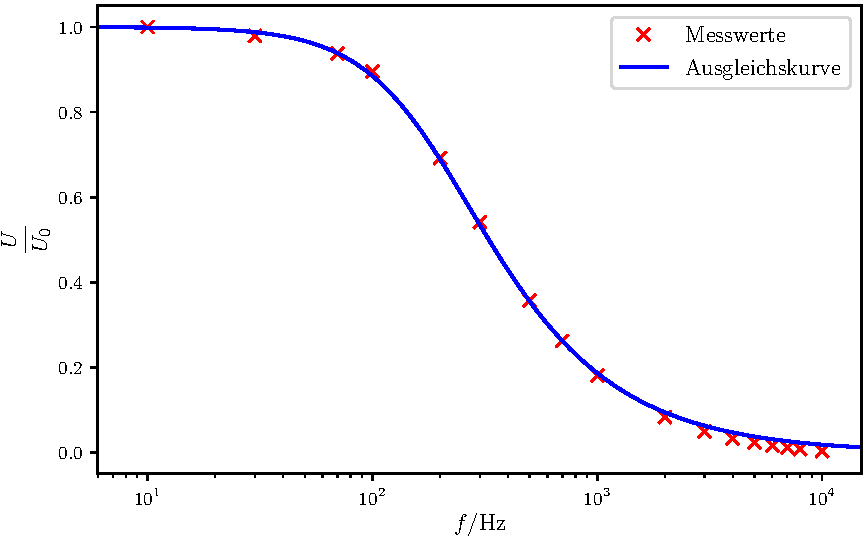
\includegraphics[width=\linewidth-100pt,height=\textheight-100pt,keepaspectratio]{content/images/Graph2.pdf}
	\caption{Die Amplitude $A$ in Abhängigkeit von der Frequenz $f$.}
	\label{fig:Graph2}
\end{figure}


\subsection{Bestimmung von RC mithilfe der Phasenverschiebung}
\label{subsec:3}
\begin{figure}
	\centering
	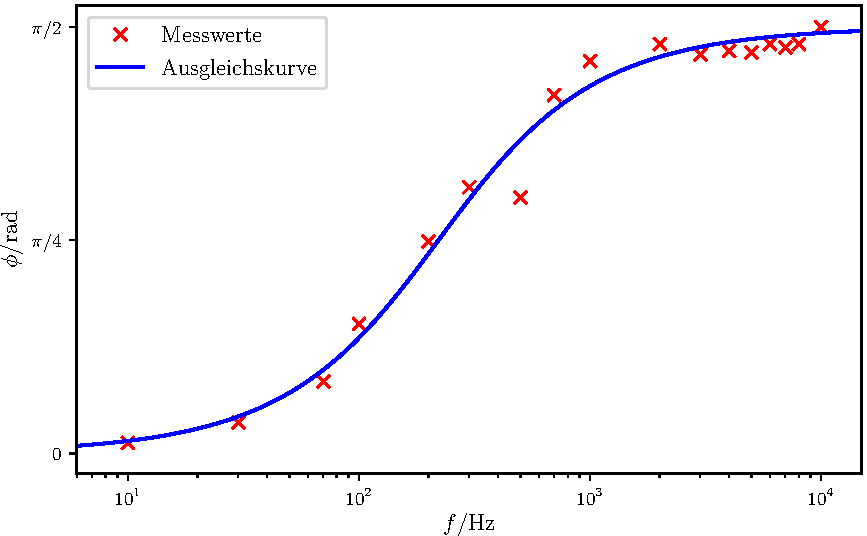
\includegraphics[width=\linewidth-100pt,height=\textheight-100pt,keepaspectratio]{content/images/Graph3.pdf}
	\caption{Die Phasenverschiebung $\phi$ in Abhängigkeit von der Frequenz $f$.}
	\label{fig:Graph3}
\end{figure}

\noindent Eine nichtlineare Ausgleichsrechnung nach Formel \eqref{eq:phi} ergibt mit den Werten aus Tabelle \ref{tab:b}:
\[
\tau = RC = \SI{4.5(3)e-3}{\second}\text{.}
\]
Dabei werden die Werte für die Phasenverschiebung $\phi$ in der Tabelle nach Formel \eqref{eq:phi1} berechnet. Der Graph ist in Abbildung \ref{fig:Graph3} dargestellt.

\subsection{Die RC-Kreis Relativamplitude in Abhängigkeit von der Phase}
\label{subsec:4}
\begin{figure}
	\centering
	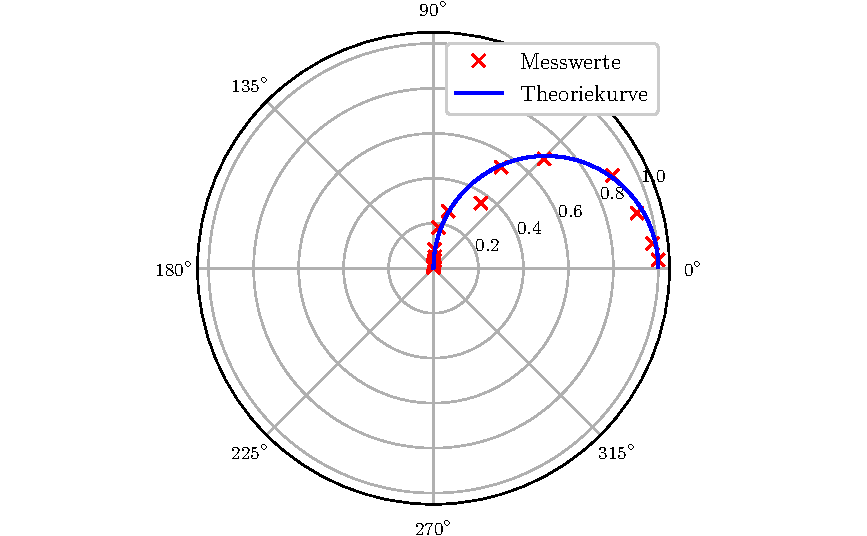
\includegraphics[width=\linewidth-70pt,height=\textheight-70pt,keepaspectratio]{content/images/Graph4.pdf}
	\caption{Die Relativamplitude $\frac{A}{U_.0}$ in Abhängigkeit von der Phasenverschiebung $\phi$.}
	\label{fig:Graph4}
\end{figure}

\noindent Nach Formel \eqref{eq:A1} und \eqref{eq:phi} ergibt sich:
\begin{equation}
\frac{A(\phi)}{U_0}=\frac{\mathrm{sin}(\phi)}{\mathrm{tan}(\phi)}=\mathrm{cos}(\phi) \label{eq:theo}
\end{equation}
In Abbildung \ref{fig:Graph4} ist die Relativamplitude $\frac{A}{U_.0}$ in einem Polardiagramm gegen die Phasenverschiebung $\phi$ aufgetragen. Die Messwerte werden Tabelle \ref{tab:b} entnommen, und die Theoriekurve wird mit dem in Abschnitt \ref{subsec:3} bestimmten $RC$ nach Formel \eqref{eq:theo} berechnet. 

\subsection{Der RC-Kreis als Integrator}
\begin{figure}
\centering
%\center{Dreieck}
\begin{minipage}{0.48\textwidth}
\centering
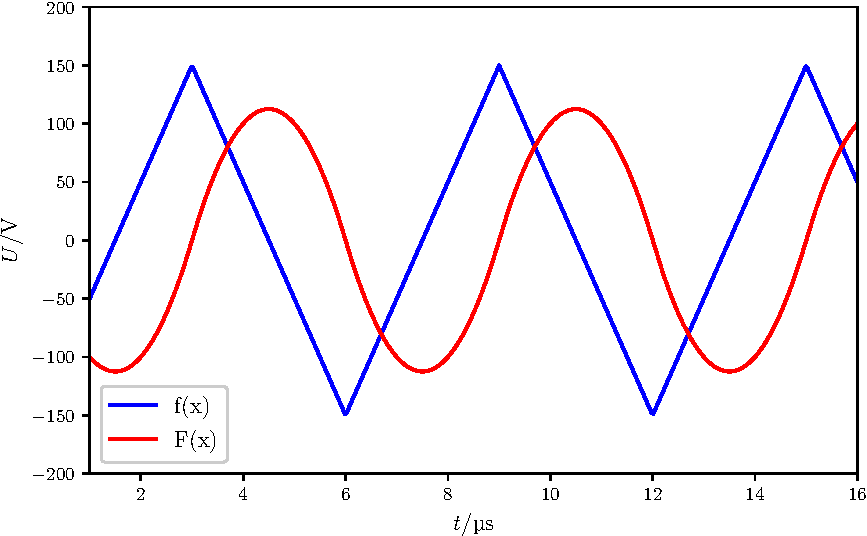
\includegraphics[width=\linewidth-10pt,height=\textheight-10pt,keepaspectratio]{content/images/Graph5.pdf}
\end{minipage}
\begin{minipage}{0.48\textwidth}
\centering
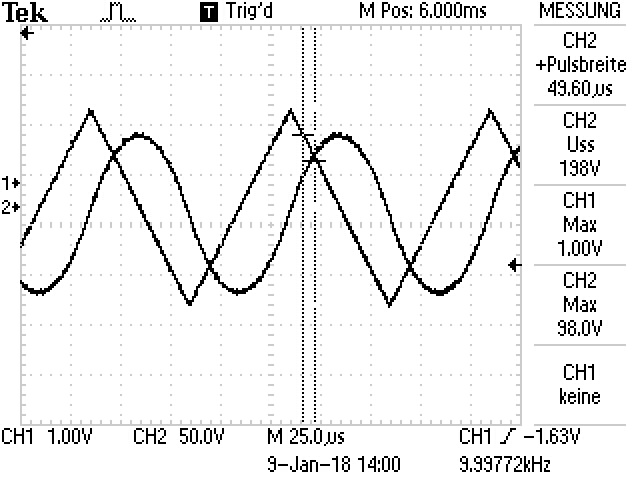
\includegraphics[width=\linewidth-10pt,height=\textheight-10pt,keepaspectratio]{content/images/5.jpg}
\end{minipage}

\vspace{2em}
%\center{Sinus}
\begin{minipage}{0.48\textwidth}
\centering
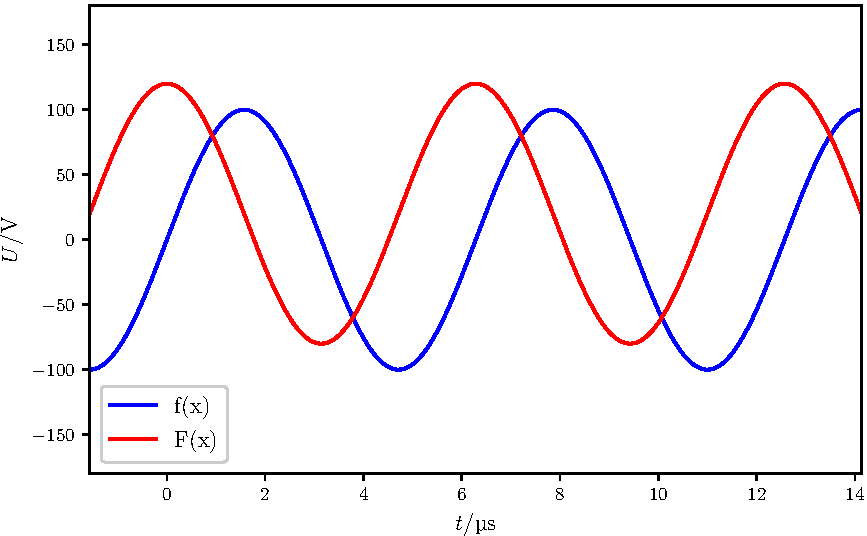
\includegraphics[width=\linewidth-10pt,height=\textheight-10pt,keepaspectratio]{content/images/Graph6.pdf}
\end{minipage}
\begin{minipage}{0.48\textwidth}
\centering
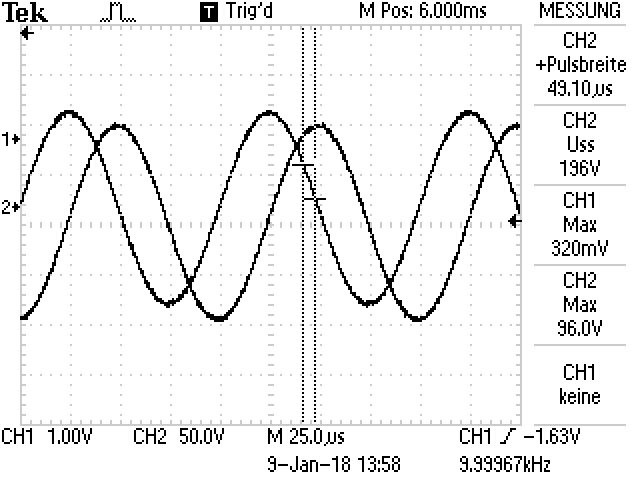
\includegraphics[width=\linewidth-10pt,height=\textheight-10pt,keepaspectratio]{content/images/6.jpg}
\end{minipage}

\vspace{2em}
%\center{Rechteck}
\begin{minipage}{.48\textwidth}
\centering
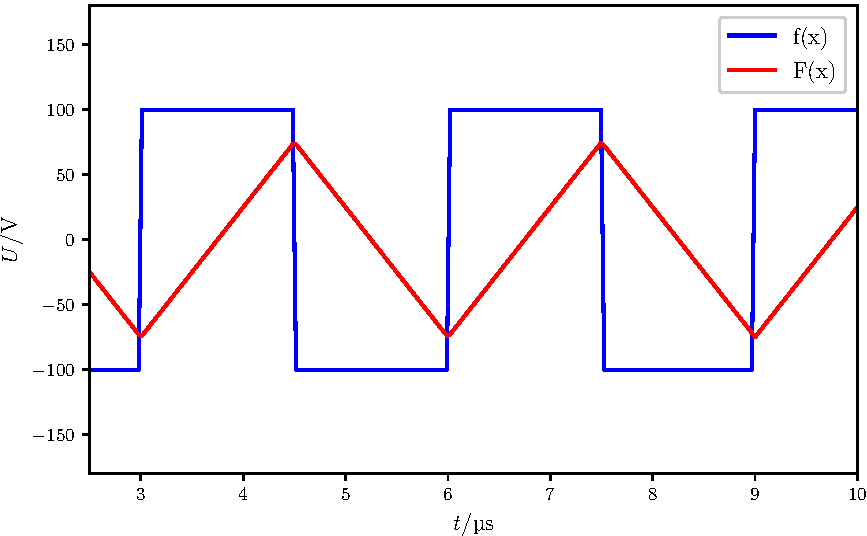
\includegraphics[width=\linewidth-10pt,height=\textheight-10pt,keepaspectratio]{content/images/Graph7.pdf}
\end{minipage}
\begin{minipage}{0.48\textwidth}
\centering
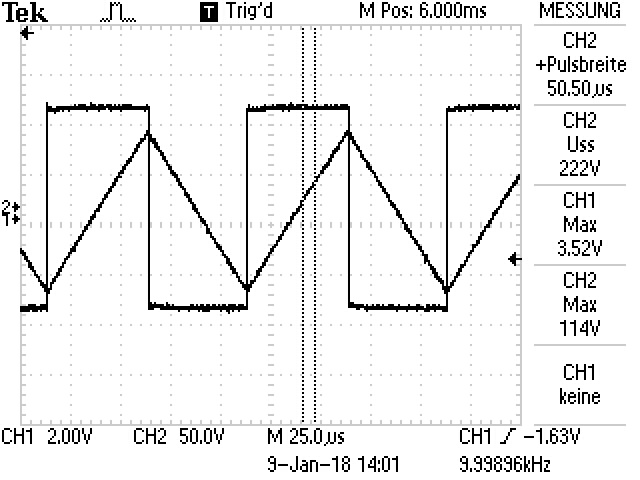
\includegraphics[width=\linewidth-10pt,height=\textheight-10pt,keepaspectratio]{content/images/7.jpg}
\end{minipage}
\caption{Beispiele für eine Dreieck-, Sinus- und Rechteckfunktion, sowie ihre Stammfunktionen im Vergleich mit den Messergebnissen}
\label{fig:U}
\end{figure}

In Abbildung \ref{fig:U} sind die Dreieck-, Sinus- und Rechteckspannung, sowie ihre Stammfunktionen im Vergleich mit theoretischen Beispiel-Funktionen abgebildet.
Die Funktion und ihre Stammfunktion der Beispiel-Dreieckspannung lauten:
\begin{align*}
f_.{Dreieck}(t)	&= 
	\begin{cases}
    A(t-\frac{T}{4})	& \text{für } nT \le t \textless \frac{T}{2}+nT\\
    A(-t+\frac{3T}{4})	& \text{für } \frac{T}{2}+nT \le t \textless nT
   	\end{cases}
\hspace{2em},n\in N \\
F_.{Dreieck}(t)	&= 
	\begin{cases}
    A(\frac{t^2}{2}-\frac{T}{4}t)					& \text{für } nT \le t \textless \frac{T}{2}+nT\\
    A(-\frac{t^2}{2}+\frac{3T}{4}t-\frac{T^2}{4})	& \text{für } \frac{T}{2}+nT \le t \textless nT
   	\end{cases}
\hspace{2em},n\in N \\
\end{align*} 
Dabei ist $A$ ein Skalierungsfaktor und $T$ stellt die Periodendauer dar. Im Beispiel beträgt $A=\SI{1e8}{\volt\per\second}$ und $T=\SI{6}{\micro\second}$. 
Die Funktion und ihre Stammfunktion der Beispiel-Sinusspannung lauten:
\begin{align*}
f_.{Sinus}(t)	&= A\sin(\omega t) \\
F_.{Sinus}(t)	&= -\frac{A}{\omega}\cos(\omega t +\pi)+C
\end{align*} 
Dabei stellt $A$ die Amplitude der Sinusspannung, $C$ die Integrationskonstante und $\omega$ die Kreisfrequenz dar. Im Beispiel beträgt $A=\SI{100}{\volt}$, $C=\SI{100}{\volt}$ und $\omega=\SI{1e6}{\per\second}$.
Die Funktion und ihre Stammfunktion der Beispiel-Rechteckspannung lauten:
\begin{align*}
f_.{Rechteck}(t)&=
	\begin{cases}
     A	& \text{für } nT \le t \textless \frac{T}{2}+nT\\
     -A  & \text{für } \frac{T}{2}+nT \le t \textless nT
   	\end{cases}
\hspace{2em},n\in N \\
F_.{Rechteck}(t)&=
	\begin{cases}
    A(t-\frac{T}{4}) 	& \text{für } nT \le t \textless \frac{T}{2}+nT\\
    -A(t+\frac{3T}{4})	& \text{für } \frac{T}{2}+nT \le t \textless nT
   	\end{cases}
\hspace{2em},n\in N \\
\end{align*} 
Dabei stellt $A$ die Amplitude der Rechteckspannung und $T$ die Periodendauer dar. Im Beispiel beträgt $A=\SI{100}{\volt}$ und $T=\SI{3}{\micro\second}$.
In allen Graphen wird die Einheit der Stammfunktion durch $\SI{1}{\micro\second}$ geteilt, um wieder eine Spannung zu erhalten.  